%%%%%%%%%%%%%%%%%%%%%%%%%%%%%%%%%%%%%%%%%%%%%%%%%%%%%%%%%%%%%%%%%%%%%%%%%%%%%%
% CONTRIBUTION TO THE MESONH BOOK1: "Convection Scheme"
% Author : Peter Bechtold
% Original : October 10, 1997
% Update   : Mai 21, 2002
%%%%%%%%%%%%%%%%%%%%%%%%%%%%%%%%%%%%%%%%%%%%%%%%%%%%%%%%%%%%%%%%%%%%%%%%%%%%%%
%
%
% DEFINITIONS:
%
% Repertoire localisant les fichiers de figure
%\documentclass[12pt]{book}
%%%%%%%%%%%%%%%%%%%%%%%%%%%%%%%%%%%%%%%%%%%%%%%%%%%%%%%%%%%
%\include{../mnh_macros.tex}
%\setcounter{page}{1}
%%%%%%%%%%%%%%%%%%%%%%%%%%%%%%%%%%%%%%%%%%%%%%%%%%%%%%%%%%%
% Repertoire localisant certains fichiers de figure
%\def\EPSDIR {eps}
%%%%%%%%%%%%%%%%%%%%%%%%%%%%%%%%%%%%%%%%%%%%%%%%%%%%%%%%%%%
%
%\begin{document}
\chapter{Convection Scheme}
\minitoc
\section{Introduction}

It has been  well recognized since the 1960s (e.g.
Charney and Eliassen 1964; Manabe and Strickler 1964; Kuo 1965;
Ooyama 1971; Yanai et al. 1973) that cumulus convection
is one of the major processes that affects the dynamics and energetics
of  atmospheric circulation systems.
Since then many cumulus parameterization schemes
 have been developed for numerical weather prediction (NWP) models and
General Circulation Models (GCMs), to account for
the subgrid-scale release of latent heat and mass transport associated
with convective clouds. A non-exhaustive list of these schemes includes e.g.
Arakawa and Schubert (1974), Anthes (1977), Kuo and Raymond (1980),
Fritsch and Chappell (1980),
Bougeault (1985), Betts and Miller (1986),
Tiedtke (1989), Gregory and Rowntree (1990), Kain and Fritsch (1990),
Emanuel (1991), Donner (1993), Grell (1993),
Wang and Randall (1996), Sun and Haines (1996), and Hu (1997).
The common point of all cumulus parameterizations is that they aim to diagnose the
presence of larger-scale conditions that would support the development of
convective activity and, under appropriate conditions, to introduce tendencies
for temperature and moisture (and possibly momentum) that would be consistent
with the effects of convective activity.  In particular, most parameterizations are
designed to drive the model atmosphere towards a convectively adjusted state
when they activate.  This adjusted state is either predefined ("adjustment"
schemes) or is computed using a bulk or spectral cloud model
and adjusting the atmosphere through mass exchange between the cloud
and the environment (mass flux schemes).

Two necessary characteristics of any convective parameterization are i) a
reasonable set of criteria to determine when convective adjustment should be
initiated, and ii) reasonable procedures for determining the characteristics of
a final convectively-adjusted state.
 In fully
prognostic dynamic models, the efficacy of a convection parameterization is
often measured by factors such as  i)  does it activate at the right time and
place?  ii)  does it produce the right amount and areal coverage of
precipitation?  and iii)  does it enhance the predictive skill of
its host model?
Of course, there are many ways of evaluating these measures, and the third
criteria above, in particular, depends on the needs of the user.  For example,
from the practical point of view of a weather forecaster, a convection scheme
used in a mesoscale model for a 1-2 day forecast provides valuable information
if it has skill in predicting the initiation and evolution of convective events,
especially if they involve severe convection.  In addition, convective
parameterization plays a critically important role in the accurate quantitative
prediction of rainfall, especially heavy rain episodes, which present a major
challenge for forecasters (Kuo et al. 1997; Fritsch et al. 1998).
In contrast, for long-range
GCM integrations a convective parameterization may be judged to be successful if
it enhances the ability of the model to accurately represent the mean climate
and variability of the tropical atmosphere. Because of these seemingly
disparate expectations, cumulus parameterizations have been developed typically
with a particular application in mind and may contain inherent biases toward
that application.

It seems reasonable, however, to expect that, to the extent that the essential
physics of convection can be represented in the crude framework of a
parameterization in a manner that is compatible with the numerics of modeling
systems, it might be possible to develop a parameterization that is useful over
a broad range of scales and type of applications.  Fundamentally, we believe
that, beyond the detection of convective activity, a primary purpose of
convective parameterization is to mitigate the effects of inappropriate
scale-selection in a modeling system's representation of deep convection.  In
particular,  we propose that if a parameterization nudges towards a reasonable
adjusted state, that its imposed time-scale of adjustment is reasonable, and
that it activates in a timely manner, it can perform well in a variety of
convective environments and model configurations.
In this context a convection parameterization has been developped
on the basis of existing frameworks,
essentially the rather general framework proposed by Kain and Fritsch (1993).
The parameterization is intended to provide an efficient representation
of atmospheric
shallow and deep convection for both mesoscale and global applications.

A detailed description of the scheme is provided below, however
 numerical applications  in different 1D, mesoscale and global contexts
are discussed in Bechtold et al. (2001) and Mallet et al. (1999).
Further 1D evaluations of the scheme
and intercomparisons with other models/schemes are presented in
Xie et al. (2002) and Bechtold et al. (2000) in the context of the international program
GCSS (GEWEX Cloud System Study).
The corresponding computer code is also available as an optimized
portable routine (both in Meso-NH and ECMWF/ARPEGE IFS code structure) in Fortran 90 on
upon request from P. Bechtold (now at ECMWF).

\section{Mass flux equations}

Briefly, with the aid of the mass flux approximation
the effect of a
convective cloud population on its environment can be written
(see e.g. Arakawa and Schubert (1974),
Gregory and Miller (1989), Betts (1997) for various derivations)

\begin{eqnarray}
{\partial\overline{\Psi}\over\partial t}\bigg\vert_{\rm conv}&=&
{\partial (\overline{ w^\prime\Psi^\prime})\over\partial z}\\
&\approx&
{1\over\overline{\rho} A } {\partial\over\partial z}
\bigg[  M^u (\Psi^u-\overline{\Psi}) + M^d (\Psi^d-\overline{\Psi})
+ \tilde M (\tilde\Psi -\overline{\Psi})\bigg]\nonumber \\
&\approx&
{1\over\overline{\rho} A } {\partial\over\partial z}
\bigg[
 M^u\Psi^u+ M^d\Psi^d-( M^u+ M^d)\overline{\Psi}
\bigg],
\label{eqc3}
\end{eqnarray}

\noindent
where $\Psi$ is a conserved variable, $M=\overline{\rho} w A$ is
the mass flux (kg s$^{-1}$), $w$ the vertical velocity, and
$A=A^u+A^d+\tilde A$  denotes the horizontal domain (grid size).
Overbars denote ensemble mean (horizontal grid mean) values, tildes
denote environmental values, up-and downdraft values are denoted
by superscripts $u$ and $d$, respectively. Furthermore,
describing the mass exchange of the cloud ensemble with its environment by
entrainment $\epsilon$ and detrainment $\delta$, i.e.

\begin{equation}
{\partial\over\partial z}  (M^u\Psi^u)=
\epsilon^u\overline{\Psi}-\delta^u\Psi^u;\quad\quad
{\partial\over\partial z}  (M^d\Psi^d)=
\epsilon^d\overline{\Psi}-\delta^d\Psi^d
\end{equation}
\noindent
we obtain the final result

\begin{eqnarray}
{\partial\overline{\Psi}\over\partial t}\bigg\vert_{\rm conv} =
{1\over\overline{\rho}^{} A }\bigg[{\partial\over\partial z}(
[ M^{u}+ M^{d}]\overline{\Psi}) -
[\epsilon^u+\epsilon^d]\overline{\Psi}+
\delta^u \Psi^{u}+\delta^d \Psi^{d}\bigg].
%[ M^{u}+ M^{d}]\overline{\Psi}) &-&
%[\epsilon^u+\epsilon^d]\overline{\Psi}^{}\nonumber\\&+&
%\delta^u \Psi^{u}+\delta^d \Psi^{d}\bigg].
\label{eqc10}
\end{eqnarray}
It can be shown that this equation is also valid for non-conserved
variables, i.e. temperature or water mixing ratios.

\section{Cloud model}

The ensemble average updraft and downdraft properties in
(\ref{eqc10}) are determined with the aid of a one-dimensional cloud model
that consists of a classical
steady-state plume convective updraft, and a corresponding
steady-state plume convective downdraft.
The cloud model is designed to represent shallow
and deep convective clouds that are characterized by their respective
cloud radius.


\subsection{Key cloud levels}

\begin{figure}
\centerline{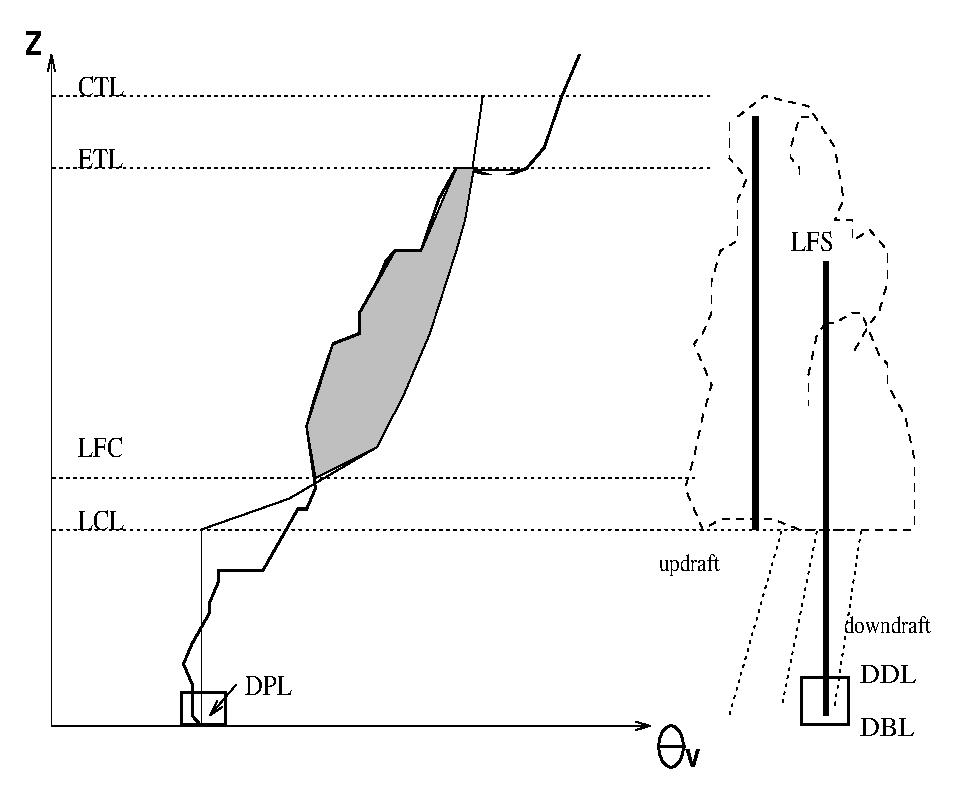
\includegraphics[width=10cm]{\EPSDIR/conv_fig1.eps}}
\caption{Environmental (thick solid line) and parcel sounding (thin solid line)
of $\theta_v$ in a deep convective cloud. The convective available
energy (CAPE) corresponds to the shaded area. The different key cloud
levels are related to condensation and buoyancy. The updraft and downdraft
regions are illustrated by the fat solid lines (the cloud is supposed
to precipitate).}
\label{conv_fig1}
\end{figure}

First, it is useful to define the
model cloud and a certain number
of important levels in the cloud that will be needed in the
following discussion. As illustrated in Fig.~\ref{conv_fig1}
the model cloud extends upward from the lifting condensation level (LCL) of
an air parcel with departure level DPL (DPL actually denotes a
60~hPa thick mixed layer) to
the cloud top level (CTL).
 The level of free convection (LFC)
is the level where the updraft becomes positively buoyant with respect
to the environment,
and the equilibrium temperature level (ETL) is
the level where the buoyancy of the updraft redrops to zero.
The convective available potential energy is defined as the positive area
(from the LFC to the ETL) between
the incloud virtual potential temperature sounding and the environmental
sounding.  The downdraft
originates within the cloud at the level of free sink (LFS), and extends down
to the downdraft base level (DBL). All downdraft mass is detrained over
a fixed layer extending from DDL to DBL.
Finally, note that the DPL and the DBL are
of course not necessarily equal to the surface level, the present figure serving
only as an example.


The following discussion of the different parts of the convection
scheme is straightforward in the way that it closely follows the sequential
structure of the scheme.



\subsection{Trigger function}

At present time, the physical processes initiating convection
are not well understood. There is no general criterion that tells
us when we should allow for convective overturning of the atmosphere; i.e.
when we should allow a moist convective parcel to overcome the stable
layer at cloud base and to have access to the CAPE that is stored aloft
due to large scale forcing associated with
e.g. midlatitude frontal systems, upper level jets or tropical waves.
However, another important
issue is the determination of the moist source layer for convection that
will be lifted up and will finally determine the properties of the
convective cloud (cloud top level, precipitation, etc.).
It turns out that over the tropical ocean this initial
moist layer corresponds to the 500-m deep boundary layer (Raymond 1995)
and the most difficult
problem is to locate the convection. However, in midlatitude convection,
especially at night time, convection might root at upper
atmospheric levels.

The numerical formalism is as follows.
Starting from the ground level, we first
construct an at least 60-hPa deep mixed layer with mean potential
temperature
$\overline{\theta}^{mix}$ and vapor mixing ratio $\overline{r}_v^{mix}$.
Then this mixed air parcel is lifted
without entrainment to its LCL.
We directly determine the temperature at the LCL using an
algorithm proposed by Davies-Jones (1983), and
compute the pressure at the LCL as
$P({\rm LCL})=P_{00}[T({\rm LCL})/\theta^{mix}]^{C_{pd}/R_d}$, where
$P_{00}$ is the reference pressure.
The air parcel is unstable with respect to moist
convection if at the LCL

\beq
\overline{\theta}_v^{mix}-\overline{\theta}_v+\Delta T/\Pi\,\,>0,
\label{dt}
\eeq
\noindent
with $\theta_v$ the virtual potential temperature, and
with the Exner function defined as $\Pi=(P/P_{00})^{R_d/C_{pd}}$. For shallow
convection the temperature increment $\Delta T$ is simply set to 0.2~K. For
deep convection $\Delta T$ is intended to crudely trigger/suppress
convection as a function of grid-scale motion, where it is defined by
$\Delta T = \pm c_{w}\,\,\,\vert \overline{w}\vert^{1/3}$,
with $c_w$=6 (K  m$^{-1/3}$ s$^{1/3}$).  The sign of $\Delta T$ is
equal to the sign of $\overline{w}$. As the large-scale vertical
velocity varies quasi-linearly as a function of the grid size, it
is normalized by $\overline{w}
\sqrt{A}/\Delta x_{ref}$,  with
$\Delta x_{ref}$ the 25-km reference grid space. Furthermore,
we test if the air parcel is able to produce a sufficient cloud depth
(at least 3~km for deep convection, and 500~m for shallow convection) by
lifting the  mixed layer parcel conserving the equivalent potential temperature
$\theta_e(\overline{\theta}^{mix},\overline{r}_v^{mix})$, and searching for the
intersection with the environmental saturated curve
$\theta_{es}(\overline{T})$ (see e.g. Raymond 1995).
If the air parcel is stable with
respect to moist convection or if its probable cloud thickness
is smaller than the specified value, the above procedure
is repeated starting at the next higher 60-hPa mixed layer, and so on.


\subsection{Updraft}

Updrafts are assumed to originate at the DPL, entrain environmental air
in the mixed layer, and then undergo undilute ascent up to the LCL.
Starting from the LCL the thermodynamic characteristics of the
updraft  are computed assuming conservation (except from
precipitation processes)
of enthalpy or "liquid water static energy" $h_{il}$ and total
water mixing ratio $r_w$

\begin{eqnarray}
h_{il}&=& C_{pm} T - L_v r_c - L_s r_i + ( 1 + r_w ) g z\label{conv-eqh}\\
r_w&=&r_v+r_c+r_i\label{conv-eqr}.
\end{eqnarray}
\noindent
where the specific heat of moist air is defined as
$C_{pm}= C_{pd} + r_w C_{pv}$, $g$ denotes the gravity constant, and
$r_v, r_c$ and $r_i$ denote the maxing ratios of water vapor and
non-precipitating cloud water/ice, respectively.
 A derivation of
$h_{il}$ is provided in the Appendix together with a definition of the
various thermodynamic constants and functions used.
The choice of $h_{il}$  is motivated by the fact
that it is linear, conserved in the presence of glaciation
processes, and easily allows to switch on/off glaciation processes in
the model.

The updraft computations are initiated at the LCL using
$h_{il}^u=C_{pm} T({\rm LCL}) + ( 1 + r_v^{mix} ) g z({\rm LCL})$ and $r_w^u=
r_v^{mix}$. The initial updraft mass flux is set to a unit value of
$M^u({\rm LCL})=\overline{\rho}\,w_{\rm LCL}\,\pi R_0^2,$
with a vertical velocity $w_{\rm LCL}$ of 1~m~s$^{-1}$ and
an updraft radius $R_0$ of 1500~m for deep and 50~m for shallow convection -
all the different parameter switches for deep and shallow convection are
summarized in Table \ref{conv-table1}.

\begin{table}
%\small
\caption{Parameters and  settings for deep and shallow convection}
\label{conv-table1}
\begin{center}
\begin{tabular}{||c|c|c||} \hline
{\bf Parameter} &{\bf deep}&\bf{shallow}\\
\hline \hline
cloud radius (m)&1500&50\\
minimum cloud thickness (m)&3000&500\\
adjustment time (h)&$0.5 < \tau<1$&3\\
$\Delta T$ (K) in "trigger"&computed from $\overline{w}$&0.2\\
downdraft&yes&no\\
precipitation&yes&no\\
\hline
\hline
\end{tabular}
\end{center}
\end{table}

Hereafter we switch to the discretized equations
on a vertical model grid $k$, with $k$ increasing with height.
The upstream operator is denoted by $\Delta\Psi=\Psi^{k+1}-\Psi^k$,
layer mean values are denoted by the additional superscript $m$.
If no superscript
is indicated we simply mean the current model level $k$. Furthermore, it
is convenient to denote the entrainment/detrainment rates $\epsilon$
and $\delta$ in mass flux units  kg s$^{-1}$ instead of units mass flux per
length as used in (\ref{eqc3})-(\ref{eqc10}).
In this notation the updraft mass flux as well as the updraft values of $h_{il}$
and $r_w$ change through mixing, detrainment and precipitation according to

\begin{eqnarray}
\Delta M^u&=&\epsilon^{um}-\delta^{um}\label{eqc0}\\
\Delta( M^u h_{il}^u)&=&\epsilon^{um}\overline{h}_{il}
-\delta^{um} h_{il}^{u} +M^{u(k+1)} (L_v \Delta r_r + L_s \Delta r_s)
\label{eqc1}\\
\Delta( M^u r_w^u)&=&\epsilon^{um}\overline{r}_w
-\delta^{um} r_w^{u}- M^{u(k+1)} (\Delta r_r + \Delta r_s).
\label{eqc2}
\end{eqnarray}

\noindent
The system (\ref{eqc0})-(\ref{eqc2}) is solved together with a
parameterization of microphysics and mixing that are described separately.

\subsubsection{Microphysics and updraft velocity}

The condensate mixing ratios  $r_c^u, r_i^u$ are deduced
from $h_{il}^u$ and $r_w^u$ using a saturation adjustment, and allowing
a gradual glaciation of the cloud in the temperature range between
268 and 248 K (see also Tao et al. 1989).
The liquid and solid precipitation
$\Delta r_r+\Delta r_s$ produced in each model layer is computed
 following Ogura and Cho (1973)
\beq
\Delta r_r+\Delta r_s=(r_c^{um}+r_i^{um}) (1- exp[-c_{pr} \Delta z/w^{um}]),
\label{eqPr}
\eeq
\noindent
where  $c_{pr}=0.02$ s$^{-1}$ is a condensate to precipitation
conversion factor. This formulation is essentially  based on the fact
that in high speed updrafts precipitation particles  do not have time to
form or are carried upward by the draft.
The updraft vertical velocity $w^u$ is evaluated with the aid of

\beq
\Delta( (w^u)^2) ={2 g\over 1+\gamma}
\left[{\theta_v^{um}-\overline{\theta}_v^m\over\overline{\theta}_v^m}\right]
\Delta z - 2{\epsilon^u\over M^u} (w^u)^2,
\label{eqc4}
\eeq
\noindent
where  $\theta_v=\theta (1+R_v/R_d\,\,r_v)/(1+r_w)$, and
$\gamma=0.5$ is the virtual mass coefficient that
approximately takes into account non-hydrostatic pressure perturbations
(Kuo and Raymond 1980).
The last term of the rhs of
(\ref{eqc4}) accounts for zero environmental momentum.
The vertical velocity is  also used to compute the cloud top level CTL,
which is defined as the level where $(w^u)^2$ becomes negative.
Finally, the total
precipitation flux produced by the updraft is simply given by
\beq
{\rm Pr}=\sum_{k={\rm LCL}}^{k={\rm CTL}}[\Delta r_r+\Delta r_s] M^u.
\eeq


\subsubsection {Entrainment and detrainment}

Unfortunately, the performance of a plume cloud model critically depends on
the specification of updraft entrainment/detrainment rates which are
functions of the cloud radius, and are generally
assumed to be constant with height. We initially adopted the
mixing formalism proposed by Kain and Fritsch (1990) where an
ensemble of mixed parcels is generated, with
positively buoyant parcels supposed to follow the cloudy updraft (entrain)
and negatively buoyant parcels supposed to detrain.
Denoting the fractional amount of environmental mass
that just yields a neutrally buoyant mixture  as $\chi_c$, the
net environmental entrainment rate and the updraft entrainment rate
are given by


\begin{eqnarray}
\epsilon^u&=&\Delta M_t\int_0^{\chi_c} \chi\,\,\, f(\chi) d\chi
\label{eqentr}\\
\delta^u&=&\Delta M_t\int^1_{\chi_c} (1-\chi) f(\chi) d\chi
\label{eqdetr}\\
\Delta M_t&=&M^u c_{\rm etr}\Delta z/R_0,
\label{eqMt}
\end{eqnarray}

\noindent
where $\Delta M_t$ with $c_{etr}=0.2$
is the total rate at which mass enters the transition
region between clear and cloudy air (Simpson 1983); $f(\chi)$ is a
Gaussian type distribution satisfying $f(0)=f(1)=0$ (Kain and Fritsch 1990).


The critical mixed fraction $\chi_c$
is solved for directly, knowing that the virtual temperature difference between
updraft-environment mixtures and that of the unmixed environment varies
linearly as a function of the environmental mass fraction $\chi$
(see Fig. \ref{conv_fig2}). The zero crossing of this curve is evaluated from

\begin{figure}
\centerline{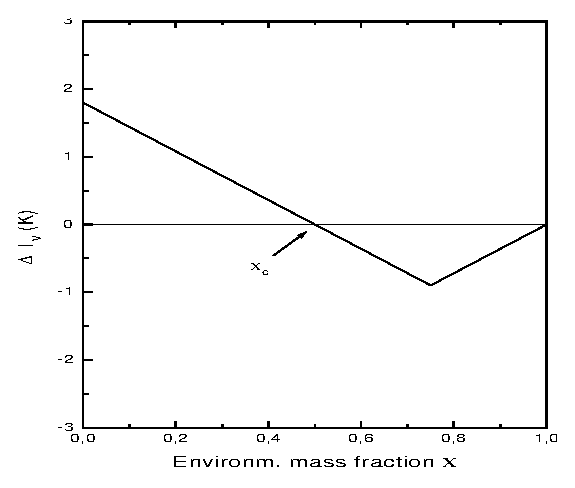
\includegraphics[width=10cm]{\EPSDIR/conv_fig2.eps}}
\caption{Plot of typical virtual temperature differences between
updraft-environment mixtures and that of the environment as a
function of the fraction of environmental mass in the mixtures.}
\label{conv_fig2}
\end{figure}

\beq
\theta_v^{mix}-\overline{\theta}_v=0=\theta_v^u-\overline{\theta}_v
- {\theta_v^u-\theta_v^{mix}\over\chi} \chi_c
\eeq
\noindent so that $\chi_c$ is given by

\beq
\chi_c={\theta_v^u-\overline{\theta}_v\over
         {\theta}_v^u-\theta_v^{mix} }   \chi; \quad \chi=0.1;
         \quad 0\le\chi_c\le 1;
\label{eqx5}
\eeq
\noindent
we use a small value of 0.1 for $\chi$ which is
supposed to be smaller than the critical value. $\theta_v^{mix}$ is
determined as a function of $h_{il}^{mix}$ and $r_w^{mix}$, where
$h_{il}^{mix}=\chi \overline{h}_{il}+(1-\chi)h_{il}^u$; idem for $r_w^{mix}$.

However, it turned out that in deep convective situations this mixing formulation often 
 produced $\epsilon^u>\delta^u$ so that the convective mass flux always increased with height,
and the upper-level mass flux was overestimated.
 Therefore, this mixing procedure was only retained for shallow convection. For deep convection
we simply use vertically constant entrainment/detrainment rates with 
 $\epsilon^u=\delta^u=0.5 \Delta M_t$.



\subsubsection{Updraft flow summary}

The updraft computations are an important
part of the convection scheme as here we build up a characteristic
precipitating cloud whose nominal mass flux is later modified
by the closure assumption. The
updraft computations can be summarized as follows:

1) Update CAPE for undilute ascent, i.e. assuming conservation of undilute
 $\theta_e$  at the LCL.

2) Estimate $r_c^u$ and $r_i^u$ at level $k+1$ setting
$h_{il}^u(k+1)=h_{il}^u(k), r_w^u(k+1)=r_w^u(k)$, and applying a
saturation adjustment procedure defined.

3) Compute $\theta_v^u(k+1)$ and square of vertical velocity using the
just computed values of $r_c^u$ and $r_i^u$ in (\ref{eqc4}).

4) Compute precipitation produced in model layer using (\ref{eqPr}).
Update total precipitation.

5) Update $r_c^u, r_i^u, h_{il}^u, r_w^u$ at level $k+1$
for precipitation.

6) Compute entrainment and detrainment rates at level $k+1$ using

7) Compute final values of updraft mass flux, $h_{il}^u, r_w^u$
at level $k+1$ using (\ref{eqc1})-(\ref{eqc2}).

8) Exit the updraft computations when the CTL is attained, i.e. when
the updraft velocity becomes negative.

9) Adjust the updraft mass flux to reflect a linear decrease of the mass
flux between the ETL and the CTL.


\subsection{Downdraft}

In contrast to the updraft computations
where condensate production and glaciation
processes are important and therefore $h_{il}$ is a very convenient
variable, the downdraft computations  become
simplified when using the equivalent potential temperature
$\theta_e$ as it implicitly takes into account the evaporational
cooling effect. The definition of $\theta_e$ is taken from Bolton (1980)
and proved to be highly accurate

\beq
\theta_e= T (P_{00}/P)^{R_d/C_{pd}(1-0.28 r_v)}
{\rm exp}[(3374.6525/T - 2.5403) r_v (1+0.81 r_v)].
\eeq

\noindent
The downdraft is assumed to be driven by cooling through melting and
evaporation of precipitation.
It originates at the level of free sink (LFS),
defined by the level of minimum environmental saturated $\theta_e$
between the LCL and the ETL.
The initial values of the downdraft mass flux, $\theta_e$ and moisture at
the LFS can be estimated as follows
\beq
M^d(LFS)= - (1-{\rm Pr_{eff}}) M^u(LCL)
\eeq

\noindent
where the precipitation efficiency Pr$_{\rm eff}$ is given as a function
of wind shear and cloud base height (Zhang and Fritsch 1986).
The initial humidity is obtained by mixing updraft and environmental air
\beq
r_w^d({\rm LFS})=\chi \overline{r}_w+(1-\chi)r_w^u; \quad
\chi=(\theta_e^u-\overline{\theta}_{es})/
(\theta_e^u-\overline{\theta}_e ).
\label{ee}
\eeq
\noindent
 This definition of the mixed fraction
 gives a very smooth variation of $\chi$, with a value
 that is close to $\chi_c$ defined in (\ref{eqx5}).
According to (\ref{ee})  the value of $\theta_e^d$ at the LFS is
set to its saturated environmental value corrected by melting effects,
with  the cooling due to melting estimated by
$\Delta T_{\rm melt}=
L_m/C_{ph}[r_w^u({\rm LCL})-r_w^u({\rm CTL})].
$
 This method is motivated by the fact
that the amount of downdraft mass flux is dependent on the total downdraft
evaporation rate which is not known initially and is itself dependent on
the magnitude of the melting effect. We know the amount of solid
precipitation but we do not know the amount of ice that is evaporated in
the downdraft.


The following equations are used to compute the downdraft properties
starting from the LFS down to the downdraft base level (DBL)
which is defined as the level where
$\theta_{e}^d(\rm{LFS}) >\overline{\theta}_{es}(\overline{T})$.


\begin{eqnarray}
\epsilon^d&=&-M^d({\rm LFS}) c_{\rm etr} \Delta z/R_0;\,\,\, k>{\rm DDL}\\
\delta^d&=&0; \quad\quad\quad\quad\quad\quad\quad\quad\quad\, k>{\rm DDL}\\
\Delta M^d&=&\epsilon^d\\
\Delta (M^d\theta_e^d)&=&\epsilon^d\overline{\theta}_e
\label{eqdt} \\
\Delta (M^d r_w^d)&=&\epsilon^d\overline{r}_w.
\label{eqdq}
\end{eqnarray}

\noindent
Note that $M^d$ is negative but $\epsilon^d$ and $\delta^d$ are positive.
All downdraft detrainment is assumed to occur over the 60~hPa
deep layer DDL-DBL (Fig. \ref{conv_fig1}).
For the closure adjustment procedure we will need the values of
$h_{il}^d$. As $\delta^d$ is zero everywhere apart from the
detrainment layer, we only
need to compute the values of $h_{il}^d$ for this layer. It is
computed from  $\theta_e^d$ and $r_w^d$.
The total downdraft evaporation rate is estimated using a specified
value of 90\% for the relative humidity. If the actual value
of humidity in the downdraft in the detrainment layer
is less than the specified
value, water is evaporated to give the required value. If no
water is evaporated, no downdraft is allowed and the
downdraft mass flux is set to zero.


\subsection{Closure}

Finally, a closure assumption is needed to control the intensity of
convection.  Here we adopt
a Fritsch Chappell type closure which is based on the assumption that all
convective available potential energy (CAPE) in a grid element is removed
within an adjustment period $\tau$. For deep convection $\tau$ is set
to the advective time period
$\tau=\sqrt{A}/\vert\vec v\vert$, with $\vec v$ the mean
horizontal wind vector between the LCL and the 500-hPa level, and is limited by
 0.5~h $< \tau <$ 1~h. The upper limit roughly corresponds to one life cycle
 of a convective cloud.
For shallow convection an adjustment time $\tau$ of 3~h is used.
With the aid of the above presented cloud model we have already
computed the initial guess updraft and downdraft mass fluxes
and the corresponding
entrainment/detrainment rates. Therefore, we are now able to compute
the final convectively-adjusted environmental values
(see also the main mass flux equations (\ref{eqc10}))
using a time integration over $\tau$ together with an iterative procedure

\begin{eqnarray}
\overline{\Psi}^{(n+1)}=\overline{\Psi}^{(n)}+(\tau/m_t)\,\,
\bigg[&-&\Delta( \tilde M^{(n)}\overline{\Psi}^{(n)})-
[\epsilon^{u(n)}+\epsilon^{d(n)}]\,\,
\overline{\Psi}^{(n)}\nonumber\\
&+&\delta^{u(n)}\Psi^{u}+\delta^{d(n)}\Psi^{d}\bigg]
\label{eqTa}
\end{eqnarray}


\beq
\tilde M=\overline{\rho}\tilde w A;\quad
\tilde w=\int(\partial\tilde w/\partial z) dz;\quad
\left({\partial\tilde{w}\over\partial z}\right)=
{\epsilon^u+\epsilon^d-\delta^u-\delta^d\over m_t},
\label{eqTb}
\eeq


\noindent
where $n$ denotes the iteration number,
$\Psi$ stands for either $h_{il}$ or the various water species  $r_w, r_c, r_i$.
The total mass of the model layer is denoted by $m_t$,
 and  $\tilde M$  is the compensating environmental mass flux.
The esssential point of the present adjustment procedure is that only
the environmental values  $\Psi= h_{il}, r_w, r_c, r_i$ are updated
and  the mass fluxes are adjusted
in the closure adjustment procedure, but no updraft or
downdraft computations are repeated so that the updraft and downdraft values
of the thermodynamic variables keep unchanged.

Now, computing the new environmental values of $\theta$ and $r_v$ from
$\overline{h}_{il}$ and $\overline{r}_w$
using (\ref{conv-eqh})-(\ref{conv-eqr}),
we can compute $\overline{\theta}_e$ and a new value of
CAPE  by using undilute parcel ascent

\begin{eqnarray}
{\rm CAPE^{(n+1)}}&=&
\int^{\rm ETL}_{\rm LCL^{(n+1)}} g
\left[ {
\overline\theta_e^{(n+1)}({\rm DPL})
\over\overline{\theta}_{es}^{(n+1)}  } -1 \right]\, dz,
\label{ecap}
\end{eqnarray}

\noindent
where the new value LCL$^{(n+1)}$ is obtained from
$\overline{\theta}_v^{(n+1)}$(DPL) by
the same procedure as used in the trigger function. The use of the
conserved variable $\overline{\theta}_{e}(DPL)$ instead of $\theta_v^u$
in (\ref{ecap}) is motivated by the fact that this formulation allows to
determine CAPE directly without executing additional updraft computations.

Then, at all model levels the updraft and downdraft mass fluxes as well as
the entrainment/detrainment fluxes and the precipitation flux
are multiplied by the adjustment factor
\beq
F_{adj}^{(n+1)}=F_{adj}^{(n)}{{\rm CAPE}^{(0)}
\over{\rm CAPE}^{(0)}-{\rm CAPE}^{(n+1)}},
\label{eqFa}
\eeq

\noindent
where ${\rm CAPE}^{(0)}$ is the initial value of CAPE.
The above described procedure
(\ref{eqTa})-(\ref{eqFa}) is repeated until
${\rm CAPE}^{(n+1)} < 0.1\,\, {\rm CAPE}^{(0)}$.
At the end of the adjustment procedure the final convective tendencies
are simply evaluated as
\beq
 {\partial\overline{\Psi}\over\partial t}\bigg\vert_{\rm conv}
 =(\overline{\Psi}^{(n)}-\overline{\Psi}^{(0)})/\tau,
\label{eqTH}
\eeq
where $\Psi$ now stands for either $\theta, r_v, r_c, r_i$.

A final remark concerns the conservation properties of the scheme, a
point that is particularly important for long time or global applications.
The scheme is designed to conserve mass and energy
as can be verified numerically from the  integral relationships

\begin{eqnarray}
\int_0^{\rm CTL}{(\epsilon^u+\epsilon^d-\delta^u-\delta^d)
\over m_t} dz = 0
\end{eqnarray}
\begin{eqnarray}
\int_{0}^{\rm CTL}  \left( {\overline{\rho}\over\rho_l}\right)
{\partial\overline{r}_w\over \partial t}\bigg\vert_{\rm conv} dz &=&
{{\rm Pr}\over \rho_l A }\\
\int_0^{\rm CTL} \left( {\overline{\rho}\over\rho_l}\right)
 {\partial\overline{h}_{il}\over\partial t}\bigg\vert_{\rm conv} dz &= &
L_v {{\rm Pr}\over \rho_l A }
\label{econs}
\end{eqnarray}

\noindent
where
 $\rho_l$ is the density of liquid water, and
${\rm Pr}\,\,\rho_l^{-1} A^{-1}$,
 is the adjusted surface precipitation flux in m s$^{-1}$.

\section{Discussion}
Our aim was to design a parameterization that incorporates the effects of the
essential physics of moist convection while remaining as straightforward and
numerically efficient as possible.  In adhering to these guidelines, however,
it is inevitable that numerous simplifications of real physical processes become
necessary.  

The limitations of a convective plume model to represent properties of a cloud ensemble
are discussed in Warner (1970), Raymond and Blyth (1986), and Lin and Arakawa (1997). 
To limit these drawbacks, we also developed an ensemble version of the code, where
the deep part can be called several times using different entrainment/detrainment rates
(=different cloud radius), and different temperature/moisture perturbations for triggering.
The resulting convective tendency is then the sum of the shallow part and the deep
convective part (which is an average of the convective tendencies and mass fluxes  of 
its individual ensemble members).



In the case of the present parameterization, an explicit dependence on
grid-length is included in two places.  First, grid-resolved vertical velocity,
as it is used in the trigger function (see discussion related to (5))
is scaled as a linear function of grid length.  Second, the convective time
period is computed as the advective time period, based on the mean wind speed in
the cloud layer and the model grid-length.  This time period is constrained to
be between 0.5 and 1 hour, however.
In addition to these implicit sensitivities to horizontal resolution, certain
physical processes have been neglected in the current parameterization.
For example, convective transport of momentum is not yet included, but could be
easily done using the scheme equations for passive tracers together with a pressure
perturbation term (Kershaw and Gregory 1997) 
Also, we do not explicitly account for mesoscale transports
that might give a substantial contribution to the mass flux at upper levels
(Donner 1993; Betts 1997; Alexander and Cotton 1998),
but the significance of this is largely unknown.
This parameterization contains several parameters that are difficult to assess.
 However, extensive testing
revealed minimal sensitivity to the values used for most of them, within a range
of reasonable values.  The most significant sensitivities appear in relation to
specification of cloud radius (determining entrainment/detrainment), the
precipitation efficiency (used to drive downdrafts), and to a lesser extent the
adjustment time scale.

Finally, lets also mention a limitation that is related to the effects of
convective downdrafts.   
In the atmosphere, convectively generated "cold pools" often spread out
over significant areas in the vicinity of thunderstorms, and the leading edge of
this cold outflow can be a region of active generation of new convective cells.
Since  prognostic variables are represented as horizontally-averaged values in
each layer within a grid-column, parameterization schemes introduce 
the effects of downdrafts as a mean cooling and drying of individual layers.
When these stabilizing tendencies are introduced as a mean effect, parameterized
convection may "turn off" due to  cooling and drying from parameterized downdrafts,
whereas in reality only a
portion of the total area represented by a grid element might experience intense
downdraft cooling. Thus 
parameterization schemes may have a tendency to
underpredict convective overturning at coarser resolutions.  A possible solution
for this problem would be to allow for partial coverage by downdraft outflow and
appropriate subgrid-scale forcing associated with outflow propagation (Liang et
al. 1998).

\section{Appendix}

\subsection{Definition of latent and specific heats}
The  specific latent heats of vaporisation, sublimation
and melting as a
function of temperature are defined by

\begin{eqnarray}
L_v(T)&=&L_v(T_t)+(C_{pv}-C_l) (T-T_t)\label{Lv}\\
L_s(T)&=&L_s(T_t)+(C_{pv}-C_s) (T-T_t)\label{Ls}\\
L_m(T)&=&L_s(T)-L_v(T)\label{Lm},
\end{eqnarray}


\noindent
with
\beq
T_t=273.16;\quad L_v(T_t)=2.5008\times 10^6
\quad L_s(T_t)=2.8345\times 10^6,
\eeq
\noindent
where $T_t$ is given in K and where the specific heats
for phase change
are given in J kg$^{-1}$. The specific heat constants
are defined as
\beq
C_{pv}=4\,\,R_v;\quad C_l=4.218\times 10^3;\quad C_s=2.106\times 10^3,
\eeq
\noindent
with $R_v$=461.525 J kg$^{-1}$ K$^{-1}$. The gas constant and specific
heat for dry air are defined as $R_d$=287.06 J kg$^{-1}$ K$^{-1}$ and
$C_{pd}= 7/2 R_d$.

\subsection{Derivation of $h_{il}$}

Following Dufour and van Mieghem (1975)  an accurate and
natural formulation of $h_{il}$ can be derived from the
enthalpy equation

\beq
C_{ph}  dT - T ( R_d + r_v R_v) d{\rm ln}P = d(L_v r_c + L_s r_i)
-\left[r_c{dL_v\over dT}+ r_i{dL_s\over dT}\right] dT,
\label{cph}
\eeq
\noindent
with $C_{ph}=C_{pd}+r_v C_{pv}+r_c C_l+r_i C_s$.
Making use of the hydrostatic approximation and the relations
(\ref{Lv})-(\ref{Lm}), (\ref{cph}) can be integrated to obtain
\beq
h_{il}= C_{pm} T - L_v r_c - L_s r_i + ( 1 + r_w ) g z,
\eeq
\noindent
with $C_{pm}= C_{pd} + r_w C_{pv}$.

\subsection{Definition of saturation mixing ratios}

The saturation pressure for water vapor over liquid water and
ice is derived from an integration of the Clausius-Clapeyron
equation

\begin{eqnarray}
e_{sl}(T)&=& exp\left[\alpha_l-{\beta_l\over T}-\gamma_l {\rm ln}(T)\right]\\
e_{si}(T)&=& exp\left[\alpha_s-{\beta_s\over T}-\gamma_s {\rm ln}(T)\right],
\end{eqnarray}

\noindent where
\beq
\alpha_l={\rm ln}[e_s(T_t)]+{\beta_l\over T_t}+\gamma_l {\rm ln}(T_t);
\quad
\beta_l={L_v(T_t)\over R_v}+\gamma_l T_t\nonumber
\label{eqab}
\eeq

\beq
\gamma_l={(C_l-C_{pv})\over R_v},
\label{eqy}
\eeq

and $e_s(T_t)=$611.14 Pa.
The corresponding coefficients for the saturation pressure over ice are
obtained by simply replacing in (\ref{eqab}) and (\ref{eqy})
the index $l$ (liquid) by the index $s$ (solid) and by replacing
$L_v$ by $L_s$.
Finally, the saturated water vapor mixing ratio is defined as
$r_{vs}(T)=(m_v/m_d) (e_s(T)/P-e_s(T)),$
with $m_v/m_d=R_d/R_v=0.622$ the ratio of dry air to water vapor Mol mass.

\subsection{Precipitation efficiency}
Defining the windshear by

\beq
S={\left\vert\vec v({\rm CTL})-\vec v ({\rm LCL})
\right\vert\over z({\rm CTL})-z({\rm LCL})}
{\vert\vec v({\rm CTL})\vert-\vert\vec v({\rm LCL})\vert\over
\big\vert\vert\vec v({\rm CTL})\vert-\vert\vec v({\rm LCL})\vert\big\vert},
\eeq

\noindent
with $\vec v$ the horizontal
wind vector, the precipitation efficiency as a function of wind shear
is expressed as

\beq
{\rm Pr_{Sef}}=1.591-0.639\, S +0.0953\, S^2-0.00496\, S^3.
\label{pref1}
\eeq

The precipitation efficiency as a function of cloud base height is
given as

\begin{eqnarray}
{\rm Pr_{Zef}}=0.967&-&0.7 z_b +1.62\times 10^{-1}z_b^2-1.26\times 10^{-2} z_b^3
\nonumber\\
&+&4.27\times 10^{-4} z_b^4-5.44\times 10^{-6} z_b^5,
\label{pref2}
\end{eqnarray}

\noindent
with $z_b$ the height difference between the LCL and the model surface level
normalized by a cloud base height of 3280~m. Both ${\rm Pr_{Sef}}$
and ${\rm Pr_{Zef}}$ are limited to values between 0.4 and 0.92.
Finally, the actual precipitation efficiency is given by
${\rm Pr_{eff}}=0.5({\rm Pr_{Sef}}+{\rm Pr_{Zef}})$.
\noindent



\section{References}
%\section*{References}

\noindent
\por
Alexander, G. D., and W.~R. Cotton, 1998:
The use of cloud resolving simulations of mesoscale convective
systems to build a mesoscale parameterization scheme.
{\it J. Atmos. Sci.}, {\bf 55}, 2137-2161.

\por
Arakawa, A., and W. H. Schubert, 1974: Interaction of a cumulus
cloud ensemble with the large-scale environment: Part I.
{\it J. Atmos. Sci.}, {\bf 31}, 674-701.

\por
Anthes, R. A., 1977: A cumulus parameterization scheme utilizing
a one-dimensional cloud model. {\it Mon. Wea. Rev.}, {\bf 105}, 270-286.

\por
Bechtold, P., E. Bazile, P. Mascart and E. Richard, 2001:
A Mass flux convection scheme for regional and global models.
{\it Quart. J. Roy. Meteor. Soc.}, {\bf 127}, 869-886.

\por
Bechtold, P., J. L. Redelsperger, I. Beau, M. Blackburn, S. Brinkop,
J. Y. Grandpeix, A. Grant, D. Gregory, F. Guichard, C. Hoff
and E. Ioannidou, 2000: A GCSS model
intercomparison for a tropical squall line observed during TOGA-COARE.
II: Intercomparison of single-column models and a cloud-resolving model.
{\it Quart. J. Roy. Meteor. Soc.}, {\bf 126}, 865-888.

\por
Betts, A. K., and M. J. Miller, 1986: A new convective adjustment scheme.
Part II: Single column tests using GATE wave, BOMEX, ATEX, and arctic air-mass
data sets. {\it Quart. J. Roy. Meteor. Soc.}, {\bf 112}, 693-709.

\por
----------, 1997:
`The parameterization of deep convection'.
In {\it "The physics and parameterization of moist atmospheric convection"}
(Ed. R. K. Smith), {\it NATO ASI Series}, {\bf 505}, 255-279.

\por
Bolton, D., 1980: The computation of equivalent potential temperature.
{\it Mon. Wea. Rev.}, {\bf 108}, 1046-1053.

\por
Bougeault, P., 1985: A simple parameterization of the large-scale
effects of cumulus convection. {\it Mon. Wea. Rev.}, {\bf 113}, 2108-2121.

\por
Bretherton, C. S., and P. K. Smolarkiewicz, 1989: Gravity waves,
compensating subsidence and detrainment around cumulus clouds.
{\it J. Atmos. Sci.}, {\bf 46}, 740-759.

%\por
%Carpenter, R. L. Jr., K. K. Droegemeier, and A. M. Blyth, 1998:
%Entrainment and detrainment in numerically simulated cumulus congestus
%clouds. Part I: General results.
%{\it J. Atmos. Sci.,} {\bf 55,} 3433-3439.

\por
Charney, J., and A. Eliassen, 1964: On the growth of the hurricane
depression. {\it J. Atmos. Sci.,} {\bf 21,} 68-75.

%\por
%Courtier, P., and J.-F. Geleyn, 1988:
%A global numerical weather prediction model with variable
%resolution: Application to the shallow-water equations.
%{\it Quart. J. Roy. Meteor. Soc.,} {\bf 114,} 1321-1346.

\por
Davies-Jones, R. P., 1983: An accurate theoretical approximation for
adiabatic condensation temperature. {\it Mon. Wea. Rev.},
{\bf 111}, 1119-1121.

\por
Donner, L. J., 1993: A cumulus parameterization including mass fluxes,
vertical momentum dynamics, and mesoscale effects.
{\it J. Atmos. Sci.}, {\bf 50}, 889-906.

\por
-----------, C. J. Seman, and R. S. Hemler, 1999: Three dimensional cloud-system
modeling of GATE convection. {\it J. Atmos. Sci.}, {\bf 56}, 1885-1912.

\por
Dufour L., and J. van Mieghem, 1975: Thermodynamique de
l'atmosph\`ere. Institut Royal M\'et\'eorologique de Belgique, 278 pp.

\por
Emanuel, K. A., 1991: A scheme for representing cumulus convection in
large-scale models. {\it J. Atmos. Sci.}, {\bf 48}, 2313-2335.

\por
----------, 1997:
The problem of convective moistening.
In {\it "The physics and parameterization of moist atmospheric convection"}
(Ed. R. K. Smith), {\it NATO ASI Series}, {\bf 505}, 447-462.
%
%\por
%Feltz, W. F., William L. Smith, Robert O. Knuteson, Henry E. Revercomb,
%Harold M. Woolf, and H. Ben Howell, 1998: Meteorological applications of
%temperature and water vapor retrievals from the ground-based Atmospheric
%Emitted Radiance Interferometer (AERI).
%{\it J.  Appl. Meteor.,} {\bf 37,} 857-875.

\por
Fritsch, J. M., and C. F. Chappell, 1980: Numerical prediction of
convectively driven mesoscale pressure systems. Part I:
Convective parameterization. {\it J. Atmos. Sci.}, {\bf 37}, 1722-1733.

\por
Fritsch, J. M., R. A. Houze, R. Adler, H. Bluestein, L. Bosart,
J. Brown, F. Carr, C. Davies, R. H. Johnson, N. Junker, Y.-H. Kuo,
S. Rutledge, J. Smith, Z. Toth, J. W. Wilson, E. Zipser, and D. Zrnic, 1998:
Quantitative precipitation forecasting: Report of the eighth prospectus
development team, U. S. weather research program.
{\it Bull. Am. Meteorol. Soc.}, {\bf 79}, 285-299.


%\por
%Grabowski, W. W., and P. K. Smolarkiewicz, 1999: CRCP: A cloud resolving
%convection parameterization for modelling the tropical convecting
%atmosphere. {\it Physica D}, to appear.

\por
Gregory, D., and M. J. Miller, 1989: A numerical study of the parameterization
of deep tropical convection. {\it Quart. J. Roy. Meteor. Soc.},
{\bf 115}, 1209-1241.

\por
Gregory, D., and P. R. Rowntree, 1990:
A mass-flux convection scheme with
representation of cloud ensemble characteristics and stability
dependent closure. {\it Mon. Wea. Rev.}, {\bf 118}, 1483-1506.

\por
Grell, G. A., 1993: Prognostic evaluation of assumptions used by
cumulus parameterizations. {\it Mon. Wea. Rev.}, {\bf 121}, 764-787.

\por
Hu, Q., 1997: A cumulus parameterization based on a cloud model of
intermittently rising thermals. {\it J. Atmos. Sci.}, {\bf 54}, 2292-2307.

\por
Kain, J. S., and J. M. Fritsch, 1990: A one-dimensional
entraining/detraining plume model and its application in
convective parameterizations. {\it J. Atmos. Sci.},
{\bf 47}, 2784-2802.

\por
-----------, and -----------, 1993: Convective parameterization for mesoscale
models: The Kain-Fritsch scheme.
{\it Meteor. Monographs}, {\bf 46}, 165-170.

\por
Kershaw, R., and D. Gregory, 1997: Parameterization of momentum
transport by convection. Part I: Theory and cloud modelling results.
{\it Quart. J. Roy. Meteor. Soc.}, {\bf 123}, 1133-1151.

%\por
%Krueger, S. K.,  D. Gregory, M. W. Moncrieff, J.-L. Redelsperger
%and W.-K. Tao, 1996:
%GCSS Working Group 4: First Cloud-Resolving Model intercomparison
%Project. Case~2.
%{\it Technical Report}, available from University of Utah, Meteorological Department.

\por
Kuo, H. L., 1965: On formation and intensification of tropical cyclones
through latent heat release by cumulus convection.
{\it J. Atmos. Sci.}, {\bf 22}, 40-63.

\por
----------, and W. H. Raymond, 1980: A quasi-one-dimensional
cumulus cloud model and parameterization of cumulus heating
and mixing effects. {\it Mon. Wea. Rev.}, {\bf 108}, 991-1009.

\por
Kuo, Y.-H., J. F. Bresch, M.-D. Cheng, J. Kain, D. B. Parsons,
W.-K. Tao and D.-L. Zhang, 1997: Summary of a mini workshop on cumulus
parameterization for mesoscale models.
{\it Bull. Am. Meteorol. Soc.}, {\bf 78}, 475-490.

%\por
%Lafore, J. P., J. Stein, N. Asencio, P. Bougeault,
%V. Ducrocq, J. Duron, C. Fischer, P. Hereil, P. Mascart,
%J. P. Pinty, J. L.  Redelsperger, E. Richard
%and J. Vila-Guerau de Arellano, 1998:
%The Meso-NH Atmospheric Simulation System.
%Part I: Adiabatic formulation and control simulations.
% {\it Annales Geophysicae}, {\bf 16}, 90-109.

%\por
%LeMone, M. A., and M. W. Moncrieff, 1993: Momentum transort by convective
%bands: Comparisons of highly idealized dynamical models to observations.
%{\it Meteor. Monographs}, {\bf 46,} 75-92.

\por
Lin, C., and A. Arakawa, 1997: The macroscopic entrainment process of simulated
cumulus ensemble. Part II: Testing the entraining-plume model
{\it J. Atmos. Sci.}, {\bf 54}, 1027-1043.

\por
Liang, Q., G. S. Young, and W. M. Frank, 1998:  A convective wake parameterization
scheme for use in general circulation models. {\it Mon. Wea. Rev.}, {\bf 126},
456-469.

\por
Mallet, I., J.-P. Cammas, P. Mascart and P. Bechtold, 1999:
Effects of cloud diabatic heating on a FASTEX cyclone (IOP17) early
development. {\it Quart. J. Roy. Meteor. Soc.}, {\bf 125}, 3415-3438.

\por Manabe, S., and R. Strickler, 1964: Thermal equilibrium
of the atmopshere with a convective adjustment.
{\it J. Atmos. Sci.}, {\bf 21}, 361-385.

\por
Mapes, B. E., 1997:
 Equilibrium versus activation control of large-scale
variations of tropical deep convection.
In {\it "The physics and parameterization of moist atmospheric convection"}
(Ed. R. K. Smith), {\it NATO ASI Series}, {\bf 505}, 321-358.

\por
Moncrieff,~M.~W., D. Gregory, S. K. Krueger, J. L. Redelsperger, and
 W. K. Tao, 1997:
 GEWEX Cloud System Study (GCSS) working group 4:
 Precipitating convective cloud systems. {\it Bull. Am. Meteorol. Soc.},
 {\bf 78}, 831-845.

\por
Ogura, Y., and H.-R. Cho, 1973: Diagnostic determination of cumulus
populations from large-scale variables. {\it J. Atmos. Sci.},
{\bf 30}, 1276-1286.

\por
Ooyama, K., 1971: A theory on parameterization of cumulus convection.
{\it J. Meteor. Soc. Japan}, {\bf 49}, 744-756.

\por
Raymond, D. J., 1995: Regulation of moist convection over the
West Pacific warm pool. {\it J. Atmos. Sci.}, {\bf 52}, 3945-3959.

\por
----------, and A. M. Blyth, 1986: A stochastic mixing model for
nonprecipitating clouds.
{\it J. Atmos. Sci.}, {\bf 43}, 2708-2718.

%\por
%Redelsperger, J. L., P. R. A; Brown, F. Guichard, C. Hoff, M. Kawasima,
%S. Lang, T. Montmerle, K. Nakamura, K. Saito, C. Seman, W. K. Tao,
%and L. J. Donner, 2000:
% A GCSS model intercomparison for a tropical squall
% line observed during TOGA-COARE. Part I: Cloud-resolving models.
%{\it Quart. J. Roy. Meteor. Soc.}, to appear.

\por
Sun, W.-H., and P. A. Haines, 1996: Semi-prognostic tests of a new cumulus
parameterization scheme for mesoscale modeling.
{\it Tellus}, {\bf 48A}, 272-289.

%\por
%S\'en\'esi, S., Bougeault, P., Ch\`eze, J.-L., Cosentino, P. and
%Thepenier, R.-M.,
%1996:
%The Vaison-la-Romaine flash flood: Mesoscale analysis and predictability
%issues. {\it Weather Forecasting,} {\bf 11,} 417-442.

%\por
%Siebesma, A. P., and J. W. M. Cuijpers, 1995: Evaluation of parametric
%assumptions for shallow cumulus convection. {\it J. Atmos. Sci.,}
%{\bf 52,} 650-666.

%\por
%----------, 1998: Shallow cumulus convection. In {\it "Buoyant convection
%in geophysical flows"} (Eds. Plate et al.), {\it Kluwer Academic Publishers,}
%441-486.

\por
Simpson, J., 1983: Cumulus clouds: interactions between laboratory
experiments and observations as foundations for models.
{\it Mesoscale Meteorology}, D. K. Lilly and T. Gal-Chen, Eds., Reidel,
399-412.

\por
Slingo, J.~M., M. Blackburn, A. K. Betts, R. Brugge, K. D. Hodges,
B. J. Hoskins, M. J. Miller, L. Steenman-Clark, and J. Thuburn, 1994:
Mean climate and
transience in the tropics of the UGAMP GCM: Sensitivity to convective
parameterization. {\it Q. J. R. Meteorol. Soc.}, {\bf 120}, 881-922.

%\por
%Stein, J., E. Richard, J. P. Lafore, J. P. Pinty, N. Ascensio and
%S. Cosma, 1999: Meso-NH simulations with grid-nesting and ice-phase
%parameterization. {\it Meteor. Atmos. Phys.}, to appear

\por
Tao, W.-K., J. Simpson, and M. McCumber, 1989: An ice-water
saturation adjustment. {\it Mon. Wea. Rev.}, {\bf 117}, 231-235.

\por
Tiedtke, M., 1989: A comprehensive mass flux scheme for cumulus
parameterization in large-scale models.
{\it Mon. Wea. Rev.}, {\bf 117}, 1779-1800.

\por
Wang, J., and D. A. Randall, 1996: A cumulus parameterization based on
the generalized convective available potential energy.
{\it J. Atmos. Sci.}, {\bf 53}, 716-727.

\por
Warner, J., 1970: On steady-state one-dimensional models of
cumulus convection. {\it J. Atmos. Sci.}, {\bf 27}, 1035-1040.

%\por
%Warner, T. T., and H.-M. Hsu, 1999: Nested model simulation of moist convection:
%The impact of coarse-grid parameterized convection on fine-grid resolved
%convection through lateral boundary effects.  {\it Mon. Wea. Rev.} to appear

\por
Xie, S.-C., K.-M. Xu, R. T. Cederwall, P. Bechtold, A. D. Del Genio, S. A. Klein,
D. G. Cripe, S. J. Ghan, D. Gregory, S. F. Iacobellis, S. K. Krueger, U. Lohmann,
J. C . Petch, D. A. Randall, L. D. Rotstayn, R. C. J. Somerville, Y. C. Sud, 
K. von Salzen, G. K. Walker, A. Wolf, J. J. Yio, G. J. Zhang and M. Zhang, 2002:
Intercomparison and evaluation of cumulus parameterizations under summertime midlatitude
continental conditions. {\it Q. J. R. Meteorol. Soc.}, {\bf 128}, 1095-1135.

\por
Yanai, M., S. K. Esbensen, and J.-H. Chu, 1973: Determination of
bulk properties of tropical cloud clusters from large-scale heat and moisture
budgets. {\it J. Atmos. Sci.}, {\bf 30}, 611-627.

\por
Zhang, D.-L., and J. M. Fritsch, 1986: Numerical simulation of the
meso-$\beta$ scale structure and evolution of the 1977 Johnstown flood.
Part I: Model description and verification. {\it J. Atmos. Sci.},
{\bf 43}, 1913-1943.

%
%%%%%%%%%%%%%%%%%%%%%%%%%%%%%%%%%%%%%%%%%%%%%%%%%%%%%%%%%%%%%%%%%%%%%%%%%
%%%%%
% END OF CONTRIBUTION TO THE MESONH BOOK1: "Convection Scheme"
%%%%%%%%%%%%%%%%%%%%%%%%%%%%%%%%%%%%%%%%%%%%%%%%%%%%%%%%%%%%%%%%%%%%%%%%%
%%%%%




%\end{document}
